%
% Chapter Introduction
%
\chapter{User Guide}
	The next chapters will guide you through the concept and the functions of DICOMUX.

\section{Workspace}
	The main concept of DICOMUX is based on the usage of workspaces. Each file or directory has its
	own workspace. If you open a Dicom file or a Dicom directory, DICOMUX will open a new workspace for
	you. The workspaces are represented as independent tabs. Modifications you do in one workspace won't    		effect any other workspace. The welcome workspace is the default one and will be shown to you
	if there are no other open workspaces.\\
	
	\begin{minipage}{\textwidth}
	\centering
	\fbox{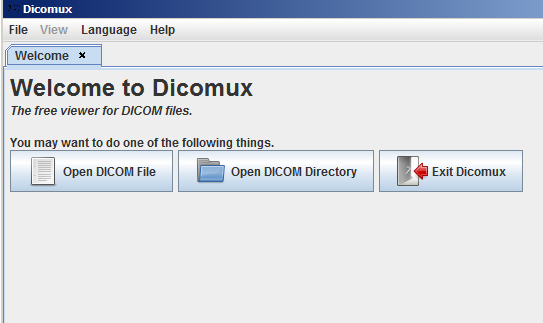
\includegraphics{screens/workspaceWelcome.png}}
	\captionof{figure}{Default workspace}
	\end{minipage}

	
	\subsection{Views}
		Each workspace, which holds an opened Dicom file, has different views. A view shows
		different parts of a dicom file. The views currently supported by DICOMUX are Raw Data, Encapsulated 			PDF, Waveform ECG and Patient Data. For example the Encapsulated PDF view shows the encapsualted pdf 		file of	an opened Dicom file. If the Dicom file doesn't have an encapsulated pdf, the view
		Encapsulated PDF won't be available.\\
	
		\begin{minipage}{\textwidth} 
		\centering
		\fbox{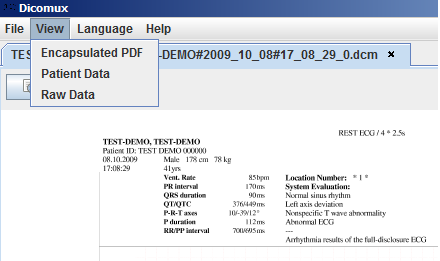
\includegraphics{screens/views.png}}
		\captionof{figure}{Switch views}
		\label{fig:bild}
		\end{minipage}

\section{Open dicom file}
	For opening a Dicom file simply click at Open Dicom File. In the following dialog, you have to select a 		Dicom file and click Open. If the chosen file is a valid Dicom file, DICOMUX loads the file into a new
	workspace. After that, you can switch between the available views.\\

	\begin{minipage}{\textwidth} 
	\centering
	\fbox{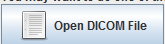
\includegraphics{screens/openFileButton.png}}
	\captionof{figure}{Open dicom file}
	\label{fig:bild}
	\end{minipage}

	\subsection{Encapsulated PDF}
		The view Encapsulated PDF shows the pdf of the Dicom file. You able to zoom into the pdf page by
		clicking the zoom button and dragging the over the pdf page. Click the zoom button again for 					resetting the zoom back to normal. \\
	
	\begin{minipage}{\textwidth} 
	\centering
	\fbox{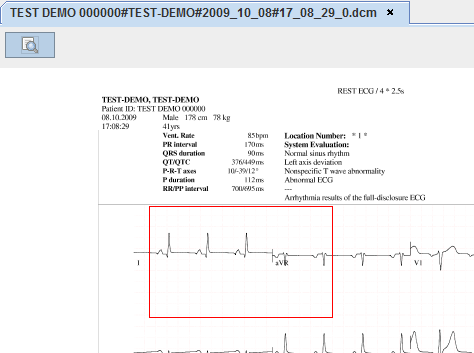
\includegraphics{screens/pdfZoomIn.png}}
	\captionof{figure}{PDF view}
	\label{fig:bild}
	\end{minipage}
	
	\subsection{Waveform ECG}
		The Waveform ECG view shows the ECG data of the Dicom file. You can zoom in
		with the plus button, zoom out with the minus button and fit to the workspace with
		the fit button. When you move the mouse over the waveforms, you can see the
		data of the current mouse position on the top panel. \\
		You will be able to select different display formats, if you open a Dicom file containing 12 lead 			ECG data.\\
		
		\begin{minipage}{\textwidth} 
		\centering
		\fbox{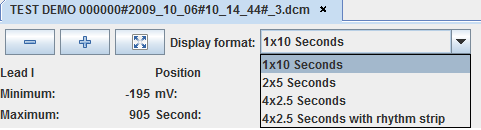
\includegraphics{screens/waveFormFormats.png}}
		\captionof{figure}{Waveform formats}
		\label{fig:bild}
		\end{minipage}
	
		\subsubsection{1x10 Seconds}
			This display format shows ten seconds of each lead in one row. All leads are
			among each other.
		
		\subsubsection{2x5 Seconds}
			This display format shows five seconds of each lead. The leads are displayed in
			two columns. the first five leads are in the first column and the second five leads
			are in the second column.\\
		
			\begin{minipage}{\textwidth} 
			\centering
			\fbox{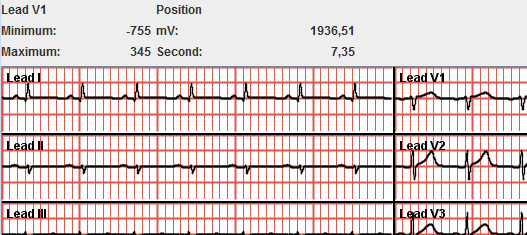
\includegraphics{screens/2x5.png}}
			\captionof{figure}{Display format 2x5}
			\label{fig:bild}
			\end{minipage}
		
		\subsubsection{4x2.5 Seconds}
			This display format shows 2.5 seconds of each lead. The leads are displayed
			in four columns. The first three leads are in the first column, the second 3
			leads are in the second column and so on.\\
		
			\begin{minipage}{\textwidth} 
			\centering
			\fbox{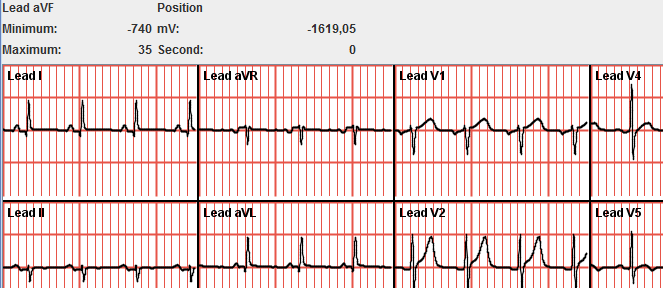
\includegraphics[scale=0.8]{screens/4x25.png}}
			\captionof{figure}{Display format 4x2.5}
			\label{fig:bild}
			\end{minipage}
		
		\subsubsection{4x2.5 Seconds with rhythm strip}
			This display format shows 2.5 seconds of each lead. The leads are displayed
			in four columns. The first three leads are in the first column, the second 3
			leads are in the second column and so on.\\
			A rhythm strip is shown at the bottom of the workspace. All 10 seconds of the rhythm
			strip are displayed in one row. \\
		
			\begin{minipage}{\textwidth} 
			\centering
			\fbox{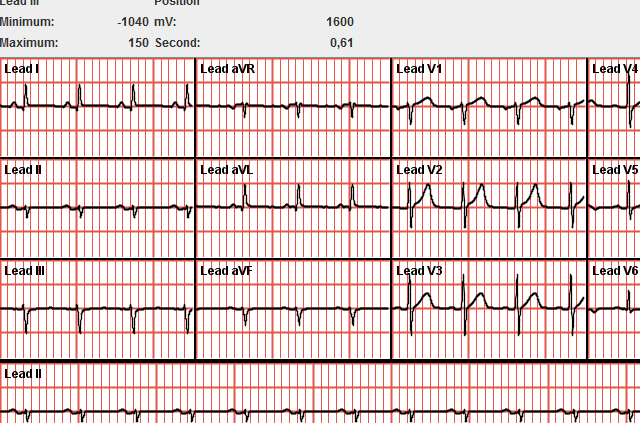
\includegraphics[scale=0.8]{screens/4x25Strip.png}}
			\captionof{figure}{Display format 4x2.5 with rhythm strip}
			\label{fig:bild}
			\end{minipage}

	\subsection{Raw Data}
		The Raw Data view shows all elements of the Dicom file in a tree with tag id, value representation,
		tag name, length and the first couple characters of the data.
		If an element contains more than one element, the view will show a folder icon next to the element 				containing the subordinated elements.\\
		After you selected an element which contains data, you can look at the entire content 							of this element by clicking on the details button at the top. If the element doesn't contain any 				data, you won't be able to look at them.\\
	
		\begin{minipage}{\textwidth} 
		\centering
		\fbox{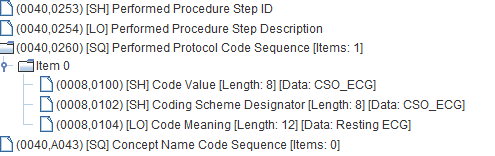
\includegraphics{screens/rawDataStructure.png}}
		\captionof{figure}{Raw data}
		\label{fig:bild}
		\end{minipage}
		
		\subsubsection{Detail view}
			The detail view displays the complete content of the previously selected element. You have the
			option to save the entire content by clicking on the save button. This makes it
			possible to save an encapsulated pdf, a report and so on in a separate file.
			To return to the Raw Data tree view, click on the return button.\\
		
			\begin{minipage}{\textwidth} 
			\centering
				\fbox{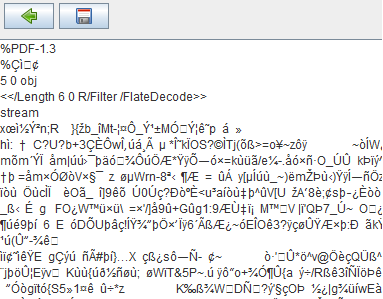
\includegraphics{screens/rawDataDetails.png}}
			\captionof{figure}{Raw data detail view}
			\label{fig:bild}
			\end{minipage}
		
	\subsection{Patient Data}
		The Patient Data view displays some information about the patient. This data will be fetched from 				the opened Dicom file.\\
	
		\begin{minipage}{\textwidth} 
		\centering
		\fbox{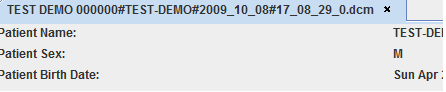
\includegraphics{screens/patientData.png}}
		\captionof{figure}{Patient details}
		\label{fig:bild}
		\end{minipage}
	
\section{Open dicom directory}
	In order to open a Dicom directory click on Open Dicom Directory and select the directory
	file. After you've selected a valid directory file, DICOMUX loads the directory
	structure into the workspace.\\
	There are four combo boxes showing patient, studies, series and images. By
	selecting an entry of a combobox you can navigate to the chosen entry.\\

	\begin{minipage}{\textwidth} 
	\centering
	\fbox{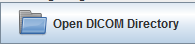
\includegraphics{screens/openDir.png}}
	\captionof{figure}{Open dicom directory}
	\label{fig:bild}
	\end{minipage}

	\subsection{Patient}
		After selecting the entry from patient, you can see the information of the
		patient. If you choose a patient, the combo boxes series and images are not
		visible anymore. For these, you have to select a study first.
	
	\subsection{Studies}
		After selecting an entry from studies, you can see the information of the chosen study.
		The combo box images is not visible. To view the images you have to
		select a series.\\
	
		\begin{minipage}{\textwidth} 
		\centering
		\fbox{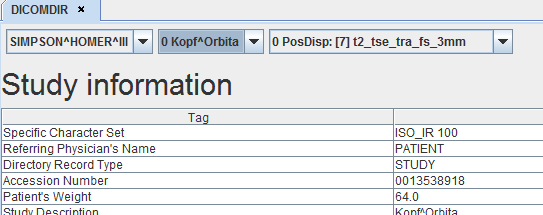
\includegraphics{screens/studyInfo.png}}
		\captionof{figure}{Study information}
		\label{fig:bild}
		\end{minipage}
	
	\subsection{Series}
		After selecting an entry from series, you can see the information of the chosen
		series. To view an images you have to select an entry of the combo box
		images.\\
	
		\begin{minipage}{\textwidth} 
		\centering
		\fbox{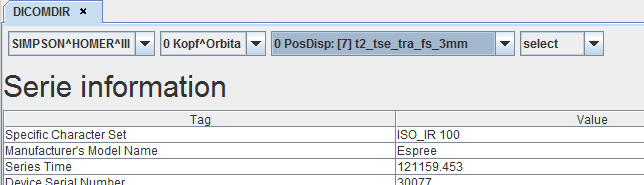
\includegraphics[scale=0.8]{screens/seriesInfo.png}}
		\captionof{figure}{Series information}
		\label{fig:bild}
		\end{minipage}
	
	\subsection{Images}
		After selecting an entry from images the chosen image will be shown to you.\\
	
		\begin{minipage}{\textwidth} 
		\centering
		\fbox{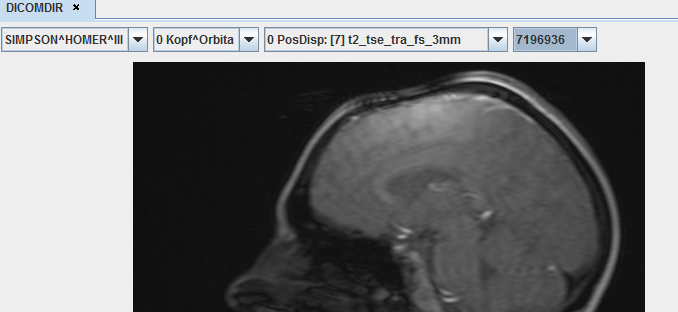
\includegraphics[scale=0.8]{screens/directoryImage.png}}
		\captionof{figure}{Directory Image}
		\label{fig:bild}
		\end{minipage}
	
\section{Language}
	DICOMUX provides multilingualism. For changing the language, goto the menu entry
	Language and select a language. After you've chosen a language, DICOMUX changes the
	language of the menu and the workspaces.\\

	\begin{minipage}{\textwidth} 
	\centering
	\fbox{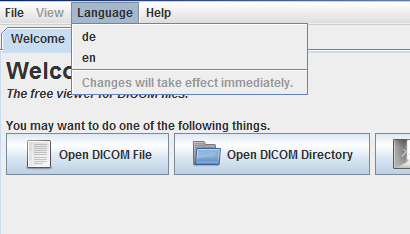
\includegraphics{screens/language.png}}
	\captionof{figure}{Change language}
	\label{fig:bild}
	\end{minipage}

%
% EOF
%